\documentclass[]{article}
\newcommand{\FileDepth}{../../..}
\usepackage[letterpaper, landscape, margin=0.5cm]{geometry}
\usepackage[T1]{fontenc}
\usepackage{textcomp}%Not strictly necessary, but gives \textmu command for "micro."
\usepackage{fancyhdr}
\usepackage{amsmath}
\usepackage{amssymb}
\usepackage{graphicx}
\usepackage{xcolor}
\usepackage{tikz}
\usetikzlibrary{calc}
\usepackage[shortlabels]{enumitem}
\usepackage{multicol}
\usepackage{vwcol}
\usepackage{hyperref}
\usepackage{wrapfig}
%opening
\newcommand{\SecType}{L}
\newcommand{\Week}{20}
\title{PH 211 Lecture \Week}
\author{Benjamin Bauml}
\date{Summer 2024}

\newcommand{\Purpose}{4}
\newcommand{\DefOnly}{0}

% Version 2024-06-14
% Changes
% 2024-02-21 Added xstring package to enable smooth implementation of new \ModePage command.
% 2024-04-27 Set up to split activities and formatting aspects into separate files. Removed dependence on xcomment. Added an automatic counter to number the activities in a problem set.
% 2024-05-19 Revised old format for \TeachingTips command, which did not support \DefOnly.
% 2024-06-14 Added Repurpose environment to allow mixing of different purpose levels in the same document.
\usepackage{tcolorbox}
\usepackage{xstring}
% You will want the following four lines in your document (the last two uncommented):
% For Assignment, leave Purpose as 1. For Worksheet, set to 2. For Student Solution, set to 3. For Teacher Solution, set to 4.
% If you want keep the pieces from being called manually, set DefOnly to 0.
%\newcommand{\Purpose}{4}
%\newcommand{\DefOnly}{1}
\newcommand{\Exclusion}{0}
\newcommand{\PageTurn}{0}
\newcommand{\GrayProb}{0}
\newcommand{\Tipsy}{0}

% Assignment
\if\Purpose1
\renewcommand{\Exclusion}{1}
\fi
% Worksheet
\if\Purpose2
\renewcommand{\Exclusion}{1}
\renewcommand{\PageTurn}{1}
\fi
% Student Solution
\if\Purpose3
\renewcommand{\PageTurn}{1}
\renewcommand{\GrayProb}{1}
\fi
% Teaching Copy
\if\Purpose4
\renewcommand{\PageTurn}{1}
\renewcommand{\GrayProb}{1}
\renewcommand{\Tipsy}{1}
\fi

\newenvironment{Repurpose}[1]{
\renewcommand{\Purpose}{#1}
\renewcommand{\Exclusion}{0}
\renewcommand{\PageTurn}{0}
\renewcommand{\GrayProb}{0}
\renewcommand{\Tipsy}{0}
% Assignment
\if\Purpose1
\renewcommand{\Exclusion}{1}
\fi
% Worksheet
\if\Purpose2
\renewcommand{\Exclusion}{1}
\renewcommand{\PageTurn}{1}
\fi
% Student Solution
\if\Purpose3
\renewcommand{\PageTurn}{1}
\renewcommand{\GrayProb}{1}
\fi
% Teaching Copy
\if\Purpose4
\renewcommand{\PageTurn}{1}
\renewcommand{\GrayProb}{1}
\renewcommand{\Tipsy}{1}
\fi
}{}

\def \NewQ {0}
\def \PForce {0}
\newcommand{\MaybePage}[1]{
	\def \PForce {#1}
	\if\PForce1
	\newpage
	\else
	\if\NewQ0
	\gdef \NewQ {\PageTurn}
	\else
	\newpage
	\fi
	\fi
}

\newcommand{\ModePage}[1]{
	\IfSubStr{#1}{\Purpose}{\newpage}{}
}

\newcounter{ActNumber}
\setcounter{ActNumber}{0}

\newcommand{\Problem}[4][0]{%The first argument is optional, and if it is set to 1, the \newpage will be forced. The second argument is the name of the activity, the third is the command the activity is stored as, and the fourth is the actual problem statement.
\newcommand{#3}{
\MaybePage{#1}
\addtocounter{ActNumber}{1}
\section*{\SecType\Week-\theActNumber: #2}
\if\GrayProb1
\begin{tcolorbox}[colback=lightgray,colframe=lightgray,sharp corners,boxsep=1pt,left=0pt,right=0pt,top=0pt,bottom=0pt,after skip=2pt]
\else
\begin{tcolorbox}[colback=white,colframe=white,sharp corners,boxsep=1pt,left=0pt,right=0pt,top=0pt,bottom=0pt,after skip=2pt]
\fi
#4
\end{tcolorbox}\noindent
}
\if\DefOnly0
\else
#3
\fi
}
	
\newcommand{\ProblemSub}[3][0]{%The first argument is optional, and if a string of numbers is entered into it, it will force a \newpage in any \Purpose that shows up in the string. For example, "13" would lead to the newpage being forced in modes 1 and 3. The second is the command the activity is stored as, and the third is the actual problem statement.
\newcommand{#2}{
\ModePage{#1}
\if\GrayProb1
\begin{tcolorbox}[colback=lightgray,colframe=lightgray,sharp corners,boxsep=1pt,left=0pt,right=0pt,top=0pt,bottom=0pt,after skip=2pt]
\else
\begin{tcolorbox}[colback=white,colframe=white,sharp corners,boxsep=1pt,left=0pt,right=0pt,top=0pt,bottom=0pt,after skip=2pt]
\fi
#3
\end{tcolorbox}\noindent
}
\if\DefOnly0
\else
#2
\fi
}
		
\newcommand{\Solution}[2]{%The first argument is the command the solution is stored as, and the second is the actual solution.
\newcommand{#1}{
\if\Exclusion0
#2
\fi
}
\if\DefOnly0
\else
#1
\fi
}
		
\newcommand{\ProblemFig}[2]{%The first argument is the command the figure is stored as, and the second is the actual figure.
\newcommand{#1}{
\begin{figure}[h]
#2
\end{figure}
}
\if\DefOnly0
\else
#1
\fi
}

\newcommand{\TeachingTips}[2]{%The first argument is the command the tip is stored as, and the second is the actual tip.
\newcommand{#1}{
\if\Tipsy1
\begin{tcolorbox}[colback=lightgray,colframe=black]
#2
\end{tcolorbox}
\fi
}
\if\DefOnly0
\else
#1
\fi
}
\usepackage[absolute]{textpos}
% This package relies on Assignment Format 2024-06-14 or later to work. It is recommended that the Purpose and DefOnly commands be given as such:
%\newcommand{\Purpose}{4}
%\newcommand{\DefOnly}{0}
% Activities need to be entered outside of the TeacherMargin and PresentSpace environments, otherwise they will be defined only locally. They can even go in the preamble.
\newenvironment{TeacherMargin}{\begin{textblock*}{10.8cm}(0.5cm,0.5cm)
\small}{\end{textblock*}
\hspace{0.1cm}}
\newenvironment{PresentSpace}{\begin{textblock*}{0.3cm}(26.85cm,9.35cm)
--
\end{textblock*}
\begin{textblock*}{0.3cm}(26.85cm,18.7cm)
--
\end{textblock*}
\begin{textblock*}{0.3cm}(26.85cm,12.24cm)
	--
\end{textblock*}
\begin{textblock*}{15.6cm}(11.8cm,0.5cm)
\begin{Repurpose}{1}
\Large}{\end{Repurpose}
\end{textblock*}
\hspace{0.1cm}}

%\newcommand{\FBDaxes}[3]{
	\begin{scope}[shift={(#1)},rotate=#2]
		% x-axis
		\draw[thick,->] (-2,0) -- (2,0);
		\node[anchor=west] at (2,0) {$x$};
		% y-axis
		\draw[thick,->] (0,-2) -- (0,2);
		\node[anchor=west] at (0,2) {$y$};
		\coordinate (#3) at (0,0);
	\end{scope}
}
\newcommand{\FBDvectorMA}[4]{
	\begin{scope}[shift={(#1)}]
		\coordinate (#4tip) at ({#2*cos(#3)},{#2*sin(#3)});
		\draw[ultra thick,blue,->] (#1) -- (#4tip);
	\end{scope}
}
\newcommand{\FBDvectorXY}[3]{
	\begin{scope}[shift={(#1)}]
		\coordinate (#3tip) at (#2);
		\draw[ultra thick,blue,->] (0,0) -- (#3tip);
	\end{scope}
}
\newcommand{\FBDdot}[1]{
	\filldraw[black] (#1) circle (3pt);
}
\newcommand{\MVec}[3][0]{%Creates a momentum vector of length #3 centered at #2 and rotated #1 degrees counterclockwise.
	\begin{scope}[rotate=#1,shift={(#2)}]
		\draw[->,thick] ({-#3/2},0) -- ({#3/2},0);
	\end{scope}
}
\newcommand{\MDot}[1]{%Creates a dot at #1 to represent a zero vector.
	\filldraw (#1) circle (1pt);
}
\newcommand{\MVDRows}[2][4.5]{%Creates the rows (initial, delta, final) of a momentum vector diagram. The optional argument determines the width of the table, and defaults to a good length for three columns (two objects and the total system). The non-optional argument gives a coordinate name (not displayed) to the diagram.
	\begin{scope}
		%\draw[thick] (0,5.5) -- (0,0);
		\draw[thick] (-1,4.5) -- (#1,4.5);
		\node at (-0.5,3.75) {$\vec{p}_{i}$};
		\draw[thick] (-1,3) -- (#1,3);
		\node at (-0.5,2.25) {$\Delta\vec{p}$};
		\draw[thick] (-1,1.5) -- (#1,1.5);
		\node at (-0.5,0.75) {$\vec{p}_{f}$};
		\coordinate (#2) at (0,5);
	\end{scope}
}
\newcommand{\MVDCol}[4][0.75]{%Creates a column for an object in a momentum vector diagram. The first (non-optional) argument is the coordinate name (not displayed) of the column, while the second is the displayed column header. The first argument also names the three entries down the column. The third argument anchors the column, so it should either be the coordinate name of the MVD (for the first column) or the coordinate name of the previous column. The optional argument indicates how far the center of the column should be from the previous column's edge, and defaults to 0.75
	\begin{scope}[shift={(#4)}]
		\node at (#1,0) {#3};
		%\draw[thick] ({#1*2},0.5) -- ({#1*2},-5);
		\draw[thick] (0,0.5) -- (0,-5);
		\coordinate (#2init) at (#1,-1.25);
		\coordinate (#2delt) at (#1,-2.75);
		\coordinate (#2fin) at (#1,-4.25);
		\coordinate (#2) at ({#1*2},0);
	\end{scope}
}

%\input{\FileDepth/Activities/Activity_One/Activity_One.tex}
%\input{\FileDepth/Activities/Activity_Two/Activity_Two.tex}

\begin{document}
\begin{TeacherMargin}

\end{TeacherMargin}
\begin{PresentSpace}
\begin{center}
	\huge Lecture \Week: Systems and Momentum
\end{center}
\vspace{0.5cm}
\underline{Project Final Drafts}
\begin{itemize}
	\item Include a reflection addressing all feedback (from me and your peers).
	\item \textbf{Cite your sources.}
	\begin{itemize}
		\item I didn't give this much attention in my feedback (a significant oversight on my part), but it is extremely important to cite your sources.
		\item Any information from outside of the course (numerical values for problems, concepts, models, equations) should be cited.
	\end{itemize}
	\item Currently due on Friday, along with Homework 7.
	\begin{itemize}
		\item Would you rather\dots
		\begin{enumerate}[(A)]
			\item Turn them both in that day.
			\item Postpone the homework due date to Sunday to focus on the project and get it done sooner.
			\item Postpone the project due date to Sunday to get the homework out of the way sooner and have more time for the project.
		\end{enumerate}
		\item Whatever you choose, I can still potentially negotiate small extensions with individual groups. However, we need things turned in early so we can give feedback and return them to you quickly before the end of the term.
	\end{itemize}
\end{itemize}
\end{PresentSpace}
\newpage
\begin{TeacherMargin}

\end{TeacherMargin}
\begin{PresentSpace}
\vspace{-10pt}
\section*{Impulse and Momentum}
\vspace{-5pt}
Definitions:
\begin{align*}
	& \text{-- Impulse} & & \vec{J}_{net} = \int_{t_{i}}^{t_{f}}\vec{F}^{net}dt \\
	& \text{-- Momentum} & & \vec{p} = m\vec{v} \\
	& \text{-- Impulse-Momentum Theorem} & & \vec{J}_{net} = \Delta\vec{p}
\end{align*}
\end{PresentSpace}
\newpage
\begin{TeacherMargin}
\begin{enumerate}[(1)]
	\item System: Both Cars \\
	For the short duration and large forces involved in a crash, the external impulse (for example, from friction with the road) would be insignificant. We can approximate conservation of momentum.
	\item System: Baseball, Catcher, 2nd Base, {\color{violet}Earth}. \\
	The forces between the catcher and 2nd base (which is firmly rooted in the Earth) probably cannot reasonably be ignored.
	\item System: Block, Spring, Table {\color{violet}Earth}. \\
	Unless the table is on frictionless wheels (which would allow it to oscillate too), it is interacting with the Earth in a significant way.
	\item System: Firework. \\
	The strong forces in a fast explosion should vastly outmatch any impulse from gravity. \\
	There is a problem in the online textbook with a firecracker that explodes over a non-negligible amount of time. Impulse cannot be ignored in that problem.
	\item System: Bird, Air, {\color{violet}Earth}. \\
	Gravity is changing the bird's momentum, and air resistance may have an appreciable effect.
\end{enumerate}
{\color{violet}Putting Earth in your system is not conducive to solving a momentum problem. Usually, it is better to leave it out to exert an impulse.}
\end{TeacherMargin}
\begin{PresentSpace}
\vspace{-10pt}
\section*{L\Week-1: Systems and Momentum Conservation}
\vspace{-5pt}
In each scenario below, if possible, identify a system for which momentum is conserved. If not possible, explain why not.
\begin{enumerate}[(1)]
	\item Two cars crash into each other in an intersection.
	\item A baseball player catches a baseball while standing at second base.
	\item A block attached to a spring on a horizontal table oscillates back and forth.
	\item A firework bursts into pieces in the sky.
	\item A bird dives through the air, speeding up.
\end{enumerate}
\end{PresentSpace}
\newpage
\begin{TeacherMargin}
\noindent\textbf{Case 1} \\
To set up a momentum vector diagram for case 1, I began with entering the initial momenta for the two cars, which told me the initial momentum for the whole system. I also assumed that momentum was conserved (by the reasoning listed in L20-1), which allowed me to fill in the 1 \& 2 column. Since the cars get tangled at the end, I know they have the same speed, and I know Car 2 is twice as big as Car 1, so it should have twice the momentum (which means it will have two thirds of the momentum of the whole system). This allowed me to fill in the rest of the final momentum row. The last two entries in the change in momentum row are now determined by the other entries in their columns.
\begin{center}
	\Large
	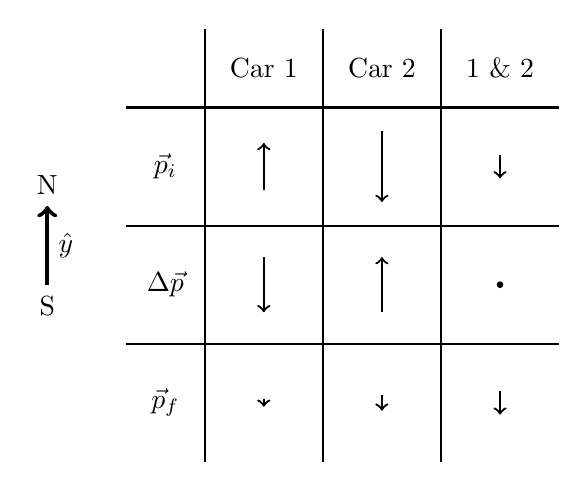
\begin{tikzpicture}
		\draw[ultra thick,->] (0,0) node[anchor=north] {S} -- (0,0.5) node[anchor=west] {$\hat{y}$} -- (0,1) node[anchor=south] {N};
		\begin{scope}[shift={(2,-2.25)}]
			\MVDRows{Caseone}
			\MVDCol{Carone}{Car 1}{Caseone}
			\MVec[90]{Caroneinit}{0.6}
			\MVec[270]{Caronedelt}{0.7}
			\MVec[270]{Caronefin}{0.1}
			\MVDCol{Cartwo}{Car 2}{Carone}
			\MVec[270]{Cartwoinit}{0.9}
			\MVec[90]{Cartwodelt}{0.7}
			\MVec[270]{Cartwofin}{0.2}
			\MVDCol{Cars}{1 \& 2}{Cartwo}
			\MVec[270]{Carsinit}{0.3}
			\MDot{Carsdelt}
			\MVec[270]{Carsfin}{0.3}
		\end{scope}
	\end{tikzpicture}
\end{center}
Already, I know that my cars should go south after the collision. Let us calculate the velocity.
\begin{align*}
	m_{1} & = 100\text{ kg} & m_{2} & = 200\text{ kg} & m_{f} & = m_{1}+m_{2} \\
	\vec{v}_{1} & = (4\text{ m/s})\hat{y} & \vec{v}_{2} & = -(3\text{ m/s})\hat{y} & \vec{v}_{f} & = v_{f}\hat{y} = ?
\end{align*}
\begin{align*}
	\vec{p}_{i} & = m_{1}\vec{v}_{1} + m_{2}\vec{v}_{2} = (m_{1}v_{1}-m_{2}v_{2})\hat{y} \\
	\vec{p}_{f} & = (m_{1} + m_{2})\vec{v}_{f} = (m_{1}+m_{2})v_{f}\hat{y}
\end{align*}
\begin{align*}
	\vec{p}_{i} & = \vec{p}_{f} & v_{f} & = \frac{m_{1}v_{1}-m_{2}v_{2}}{m_{1}+m_{2}} \\
	m_{1}v_{1} - m_{2}v_{2} & = (m_{1}+m_{2})v_{f} &  & = \frac{(100\text{ kg})(4\text{ m/s})-(200\text{ kg})(3\text{ m/s})}{100\text{ kg}+200\text{ kg}} \\
	& & & = \frac{400-600}{300}\text{ m/s} = -\frac{2}{3}\text{ m/s}
\end{align*}
\begin{align*}
	K_{i} & = \frac{1}{2}m_{1}v_{1}^{2} + \frac{1}{2}m_{2}v_{2}^{2} \\
	& = \frac{1}{2}(100\text{ kg})(4\text{ m/s})^{2} + \frac{1}{2}(200\text{ kg})(3\text{ m/s})^{2} = 800\text{ J} + 900\text{ J} = 1700\text{ J} \\
	K_{f} & = \frac{1}{2}(m_{1}+m_{2})v_{f}^{2} = \frac{1}{2}(300\text{ kg})\left(\frac{2}{3}\text{ m/s}\right)^{2} = \frac{200}{3}\text{ J} \approx 66.7\text{ J}
\end{align*}
A lot of energy is lost to heat and deformation of metal.
\end{TeacherMargin}
\begin{PresentSpace}
\vspace{-10pt}
\section*{L\Week-2: Bumper Cars}
\vspace{-10pt}
\begin{itemize}
	\item Two bumper cars collide with each other and get tangled together.
	\item Car 1 ($m_{1}$) moves north at $v_{1}$. Car 2 ($m_{2}$) moves south at $v_{2}$.
\end{itemize}
\begin{multicols}{2}
	\begin{itemize}
		\item Case 1
		\begin{itemize}
			\large
			\item Car 1 (100 kg) moves north at 4 m/s.
			\item Car 2 (200 kg) moves south at 3 m/s.
			\item Find the final velocity of the cars.
			\item Determine the initial and final kinetic energies of the cars.
			\item Compare the total kinetic energy before and after the collision.
		\end{itemize}
		\item Case 2
		\begin{itemize}
			\large
			\item Car 1 (100 kg) moves north at 4 m/s.
			\item Car 2 (200 kg) moves south.
			\item Find the initial velocity of Car 2 assuming they both end at rest.
			\item Determine the initial and final kinetic energies of the cars.
			\item Compare the total kinetic energy before and after the collision.
		\end{itemize}
	\end{itemize}
\end{multicols}
\end{PresentSpace}
\newpage
\begin{TeacherMargin}
\noindent\textbf{Case 2} \\
To set up a momentum vector diagram for case 2, I began with entering the initial momentum for Car 1, along with the entire final momentum row (which is all zero). for the two cars, which told me the initial momentum for the whole system. I also assumed that momentum was conserved (by the reasoning listed in L20-1), which allowed me to fill in the 1 \& 2 column with more zeros. The zero final momentum in the Car 1 column let me fill in the first car's change in momentum, then the zeros in the 1 \& 2 column helped me to fill in the momenta for Car 2.
\begin{center}
	\Large
	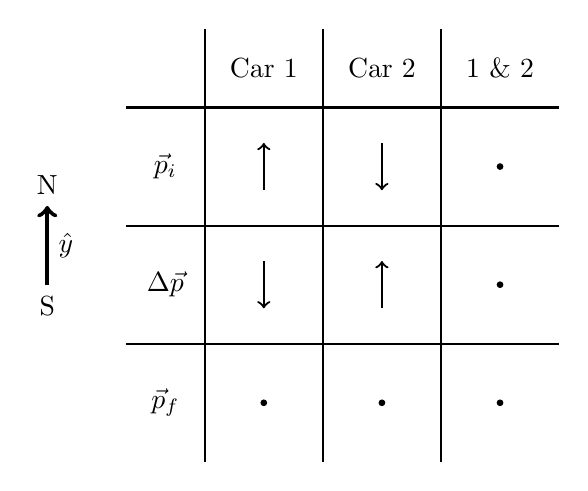
\begin{tikzpicture}
		\draw[ultra thick,->] (0,0) node[anchor=north] {S} -- (0,0.5) node[anchor=west] {$\hat{y}$} -- (0,1) node[anchor=south] {N};
		\begin{scope}[shift={(2,-2.25)}]
			\MVDRows{Caseone}
			\MVDCol{Carone}{Car 1}{Caseone}
			\MVec[90]{Caroneinit}{0.6}
			\MVec[270]{Caronedelt}{0.6}
			\MDot{Caronefin}
			\MVDCol{Cartwo}{Car 2}{Carone}
			\MVec[270]{Cartwoinit}{0.6}
			\MVec[90]{Cartwodelt}{0.6}
			\MDot{Cartwofin}
			\MVDCol{Cars}{1 \& 2}{Cartwo}
			\MDot{Carsinit}
			\MDot{Carsdelt}
			\MDot{Carsfin}
		\end{scope}
	\end{tikzpicture}
\end{center}
Already, I know that the second car must have equal and opposite initial momentum to the first car.
\begin{align*}
	m_{1} & = 100\text{ kg} & m_{2} & = 200\text{ kg} & m_{f} & = m_{1}+m_{2} \\
	\vec{v}_{1} & = (4\text{ m/s})\hat{y} & \vec{v}_{2} & = -v_{2}\hat{y} = ? & \vec{v}_{f} & = \vec{0}
\end{align*}
\begin{align*}
	\vec{p}_{i} & = m_{1}\vec{v}_{1} + m_{2}\vec{v}_{2} = (m_{1}v_{1}-m_{2}v_{2})\hat{y} \\
	\vec{p}_{f} & = (m_{1} + m_{2})\vec{v}_{f} = \vec{0}
\end{align*}
\begin{align*}
	\vec{p}_{i} & = \vec{p}_{f} & v_{2} & = \frac{m_{1}}{m_{2}}v_{1} \\
	m_{1}v_{1} - m_{2}v_{2} & = 0 &  & = \frac{1}{2}v_{1} \\
	& & & = 2\text{ m/s}
\end{align*}
Car 2 was going 2 m/s (to the south). They both end at rest, so $K_{f}=0$ J.
\begin{align*}
	K_{i} & = \frac{1}{2}m_{1}v_{1}^{2} + \frac{1}{2}m_{2}v_{2}^{2} \\
	& = \frac{1}{2}(100\text{ kg})(4\text{ m/s})^{2} + \frac{1}{2}(200\text{ kg})(2\text{ m/s})^{2} = 800\text{ J} + 400\text{ J} = 1200\text{ J}
\end{align*}
All of the energy was lost to heat and deformation of metal.
\end{TeacherMargin}
\begin{PresentSpace}
\vspace{-10pt}
\section*{L\Week-2: Bumper Cars}
\vspace{-10pt}
\begin{itemize}
	\item Two bumper cars collide with each other and get tangled together.
	\item Car 1 ($m_{1}$) moves north at $v_{1}$. Car 2 ($m_{2}$) moves south at $v_{2}$.
\end{itemize}
\begin{multicols}{2}
	\begin{itemize}
		\item Case 1
		\begin{itemize}
			\large
			\item Car 1 (100 kg) moves north at 4 m/s.
			\item Car 2 (200 kg) moves south at 3 m/s.
			\item Find the final velocity of the cars.
			\item Determine the initial and final kinetic energies of the cars.
			\item Compare the total kinetic energy before and after the collision.
		\end{itemize}
		\item Case 2
		\begin{itemize}
			\large
			\item Car 1 (100 kg) moves north at 4 m/s.
			\item Car 2 (200 kg) moves south.
			\item Find the initial velocity of Car 2 assuming they both end at rest.
			\item Determine the initial and final kinetic energies of the cars.
			\item Compare the total kinetic energy before and after the collision.
		\end{itemize}
	\end{itemize}
\end{multicols}
\end{PresentSpace}
\newpage
\begin{TeacherMargin}
	
\end{TeacherMargin}
\begin{PresentSpace}
\section*{Main Ideas}
\begin{itemize}
	\item Momentum and impulse are useful quantities for solving dynamics problems.
	\item The impulse is always equal to the change in momentum for a system.
	\item When the impulse is zero (because the net force is zero), the momentum of the system is constant---it is \textit{conserved}.
\end{itemize}
\end{PresentSpace}
\end{document}